\باب{ترچی آمد، انعکاس، انحراف اور  انکسار}
دو خطوں کے سرحد پر عمودی آمدی موج کے انعکاس اور ترسیل پر باب \حوالہ{باب_مستوی_امواج} میں غور کیا گیا۔اس باب میں ترچی آمدی موج کی بات کرتے ہوئے انعکاس اور ترسیل کے علاوہ انحراف اور انکسار کی بھی بات کی جائے گی۔عمودی امواج اور ترسیسلی تار کے مساوات ہوبہو ایک جیسے تھے۔ ترچی آمدی موج کی مساوی مثال ترسیلی تار میں نہیں پائی جاتی۔یہی وجہ ہے کہ ان پر یہاں علیحدہ  غور کیا جا رہا ہے۔

\حصہ{ترچی آمد}
شکل میں سرحد پر ترچی آمد موج دکھائی گئی ہے۔سرحد \عددیء{y=0} سطح پر پایا جاتا ہے لہٰذا \عددیء{y} محدد، سرحد کے عمودی ہے۔پہلے خطے (خطہ-1) میں آمدی برقی موج \عددیء{y} محدد کے ساتھ \عددیء{\theta_i} زاویہ بناتا ہے جبکہ اسی خطے میں انعکاسی برقی موج \عددیء{y} محدد کے ساتھ \عددیء{\theta_r} زاویہ بناتا ہے۔ترسیلی موج دوسرے خطے (خطہ-2) میں منفی \عددیء{y} محدد کے ساتھ \عددیء{\theta_t} زاویہ بناتا ہے۔
\begin{figure}
\centering
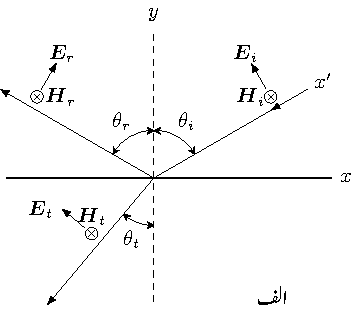
\includegraphics{figObliqueIncidenceParallelElectricField}
\caption{ترچی آمد کی صورت میں انعکاسی اور ترسیلی امواج اور ان کے زاویے۔برقی میدان سطح سرحد کے متوازی ہے۔}
\label{شکل_ترچی_آمد_متوازی_برقی_میدان_عمومی_شکل}
\end{figure}

\begin{figure}
\centering
\includegraphics{figObliqueIncidenceParallelElectricFieldCoordinateTransformation}
\caption{}
\label{شکل_ترچی_محدد_کی_تبدیلی}
\end{figure}
